\documentclass[format=acmsmall, review=false, screen=true]{acmart}

\usepackage{booktabs} % For formal tables
\usepackage{upgreek}
\usepackage[ruled]{algorithm2e} % For algorithms
\renewcommand{\algorithmcfname}{ALGORITHM}
\SetAlFnt{\small}
\SetAlCapFnt{\small}
\SetAlCapNameFnt{\small}
\SetAlCapHSkip{0pt}
\IncMargin{-\parindent}


% Metadata Information
\acmJournal{TWEB}
\acmVolume{9}
\acmNumber{4}
\acmArticle{39}
\acmYear{2018}
\acmMonth{3}
\copyrightyear{2018}
%\acmArticleSeq{9}

% Copyright
%\setcopyright{acmcopyright}
\setcopyright{acmlicensed}
%\setcopyright{rightsretained}
%\setcopyright{usgov}
%\setcopyright{usgovmixed}
%\setcopyright{cagov}
%\setcopyright{cagovmixed}

% DOI
%\acmDOI{0000001.0000001}

% Paper history
%\received{February 2007}
%\received[revised]{March 2009}
%\received[accepted]{June 2009}


% Document starts
\begin{document}
% Title portion. Note the short title for running heads
\title[]{DoubleM-KV: A Distributed RDMA-enabled Persistent Memory Key-Value Store with Low Latency and Fast Replication}

\author{Hao Liu}
\orcid{0000-0003-3026-478X}
\affiliation{
	\institution{Tsinghua University}
	\streetaddress{30 Shuangqing Road}
	\city{Haidian District}
	\state{Beijing City}
	\country{China}
}
\email{haoliu@tsinghua.edu.cn}

\author{Youyou Lu}
\affiliation{
	\institution{Tsinghua University}
	\streetaddress{30 Shuangqing Road}
	\city{Haidian District}
	\state{Beijing City}
	\country{China}
}
\email{luyouyou@tsinghua.edu.cn}

\author{Jiwu Shu}
\affiliation{
	\institution{Tsinghua University}
	\streetaddress{30 Shuangqing Road}
	\city{Haidian District}
	\state{Beijing City}
	\country{China}
}
\email{shujw@tsinghua.edu.cn}

\begin{abstract}

	Emerging non-volatile memory(NVM) medium brings revolutionary impact on storage technology landscape. Well-combination of byte-addressability and non-volatility features and comparable performance with DRAM make NVM become a competitive choice for both working memory and persistent storage. RDMA which stands for remote direct memory access is a direct memory access technology from the memory of one computer into that of another without involving either one's operating system. It permits high-throughput, low-latency networking, and has already existed for decades in server clusters and data centers. The promising of NVM makes RDMA technology popular again because the combination of these two technologies offers a clear possibility of constructing a high throughput, low latency and large volume persistent storage platform, such as distributed persistent memory file system and key-value store system. In this paper, we explore the design and implementation of a distributed key-value store system which utilizing both of NVM and RDMA. Our prototype system calls DoubleM-KV, it collects modifications of both data and meta data at the local NVM of the primary server and replicate them to the same positions of backup servers by RDMA writes. Extensive experiment shows that DoubleM-KV achieves significant latency	reduction and fast replication of user data. It stores a 32 bytes key-value pair with a replication degree of 3 in less than 2$\upmu$s and the whole request latency is less than 10$\upmu$s which is only 20\% of that Memcached's request latency under IPoIB protocol.

\end{abstract}

%
% The code below should be generated by the tool at
% http://dl.acm.org/ccs.cfm
% Please copy and paste the code instead of the example below.
%
\begin{CCSXML}

\end{CCSXML}
\ccsdesc[500]{Computer systems organization~Storage systems}
\ccsdesc[300]{Computer systems organization~Replication}

%
% End generated code
%

\keywords{Non-Volatile Memory, Key-Value Store, RDMA, Fast Replication}

\maketitle

% The default list of authors is too long for headers.
%\renewcommand{\shortauthors}{G. Zhou et al.}
%\section{Introduction}


As a new technology, Wireless Sensor Networks (WSNs) has a wide
range of applications \cite{Culler-01, Bahl-02, Akyildiz-01}, including
environment monitoring, smart buildings, medical care, industrial and
military applications. Among them, a recent trend is to develop
commercial sensor networks that require pervasive sensing of both
environment and human beings, for example, assisted living
\cite{Akyildiz-02, Harvard-01,CROSSBOW} and smart homes
\cite{Harvard-01, Adya-01,CROSSBOW}.
% quote
\begin{quote}
  ``For these applications, sensor devices are incorporated into human
  cloths \cite{Natarajan-01, Zhou-06, Bahl-02, Adya-01} for monitoring
  health related information like EKG readings, fall detection, and
  voice recognition''.
\end{quote}
While collecting all these multimedia information
\cite{Akyildiz-02} requires a high network throughput, off-the-shelf
sensor devices only provide very limited bandwidth in a single
channel: 19.2\,Kbps in MICA2 \cite{Bahl-02} and 250\,Kbps in MICAz.

In this article, we propose MMSN, abbreviation for Multifrequency
Media access control for wireless Sensor Networks. The main
contributions of this work can be summarized as follows.
% itemize
\begin{itemize}
\item To the best of our knowledge, the MMSN protocol is the first
multifrequency MAC protocol especially designed for WSNs, in which
each device is equipped with a single radio transceiver and
the MAC layer packet size is very small.
\item Instead of using pairwise RTS/CTS frequency negotiation
\cite{Adya-01, Culler-01, Tzamaloukas-01, Zhou-06},
we propose lightweight frequency assignments, which are good choices
for many deployed comparatively static WSNs.
\item We develop new toggle transmission and snooping techniques to
enable a single radio transceiver in a sensor device to achieve
scalable performance, avoiding the nonscalable ``one
control channel + multiple data channels'' design \cite{Natarajan-01}.
\end{itemize}

% Head 1
\section{MMSN Protocol}

% Head 2
\subsection{Frequency Assignment}

We propose a suboptimal distribution to be used by each node, which is
easy to compute and does not depend on the number of competing
nodes. A natural candidate is an increasing geometric sequence, in
which
% Numbered Equation
\begin{equation}
\label{eqn:01}
P(t)=\frac{b^{\frac{t+1}{T+1}}-b^{\frac{t}{T+1}}}{b-1},
\end{equation}
where $t=0,{\ldots}\,,T$, and $b$ is a number greater than $1$.

In our algorithm, we use the suboptimal approach for simplicity and
generality. We need to make the distribution of the selected back-off
time slice at each node conform to what is shown in
Equation~\eqref{eqn:01}. It is implemented as follows: First, a random
variable $\alpha$ with a uniform distribution within the interval $(0,
1)$ is generated on each node, then time slice $i$ is selected
according to the following equation:
% Unnumbered Equation
\[
i=\lfloor(T+1)\log_b[\alpha(b-1)+1]\rfloor.
\]
It can be easily proven that the distribution of $i$ conforms to Equation
(\ref{eqn:01}).

So protocols \cite{Bahl-02, Culler-01,Zhou-06,Adya-01,
Tzamaloukas-01, Akyildiz-01} that use RTS/CTS
controls\footnote{RTS/CTS controls are required to be implemented by
802.11-compliant devices. They can be used as an optional mechanism
to avoid Hidden Terminal Problems in the 802.11 standard and
protocols based on those similar to \cite{Akyildiz-01} and
\cite{Adya-01}.} for frequency negotiation and reservation are not
suitable for WSN applications, even though they exhibit good
performance in general wireless ad-hoc
networks.

% Head 3
\subsubsection{Exclusive Frequency Assignment}


In exclusive frequency assignment, nodes first exchange their IDs
among two communication hops so that each node knows its two-hop
neighbors' IDs. In the second broadcast, each node beacons all
neighbors' IDs it has collected during the first broadcast period.

% Head 4
\paragraph{Eavesdropping}

Even though the even selection scheme leads to even sharing of
available frequencies among any two-hop neighborhood, it involves a
number of two-hop broadcasts. To reduce the communication cost, we
propose a lightweight eavesdropping scheme.

\subsection{Basic Notations}

As Algorithm~\ref{alg:one} states, for each frequency
number, each node calculates a random number (${\textit{Rnd}}_{\alpha}$) for
itself and a random number (${\textit{Rnd}}_{\beta}$) for each of its two-hop
neighbors with the same pseudorandom number generator.

% Algorithm
\begin{algorithm}[t]
\SetAlgoNoLine
\KwIn{Node $\alpha$'s ID ($ID_{\alpha}$), and node $\alpha$'s
neighbors' IDs within two communication hops.}
\KwOut{The frequency number ($FreNum_{\alpha}$) node $\alpha$ gets assigned.}
$index$ = 0; $FreNum_{\alpha}$ = -1\;
\Repeat{$FreNum_{\alpha} > -1$}{
        $Rnd_{\alpha}$ = Random($ID_{\alpha}$, $index$)\;
        $Found$ = $TRUE$\;
        \For{each node $\beta$ in $\alpha$'s two communication hops
    }{
      $Rnd_{\beta}$ = Random($ID_{\beta}$, $index$)\;
      \If{($Rnd_{\alpha} < Rnd_{\beta}$) \text{or} ($Rnd_{\alpha}$ ==
          $Rnd_{\beta}$ \text{and} $ID_{\alpha} < ID_{\beta}$)\;
      }{
        $Found$ = $FALSE$; break\;
      }
        }
     \eIf{$Found$}{
           $FreNum_{\alpha}$ = $index$\;
         }{
           $index$ ++\;
     }
      }
\caption{Frequency Number Computation}
\label{alg:one}
\end{algorithm}


Bus masters are divided into two disjoint sets, $\mathcal{M}_{RT}$
and $\mathcal{M}_{NRT}$.
% description
\begin{description}
\item[RT Masters]
$\mathcal{M}_{RT}=\{ \vec{m}_{1},\dots,\vec{m}_{n}\}$ denotes the
$n$ RT masters issuing real-time constrained requests. To model the
current request issued by an $\vec{m}_{i}$ in $\mathcal{M}_{RT}$,
three parameters---the recurrence time $(r_i)$, the service cycle
$(c_i)$, and the relative deadline $(d_i)$---are used, with their
relationships.
\item[NRT Masters]
$\mathcal{M}_{NRT}=\{ \vec{m}_{n+1},\dots,\vec{m}_{n+m}\}$ is a set
of $m$ masters issuing nonreal-time constrained requests. In our
model, each $\vec{m}_{j}$ in $\mathcal{M}_{NRT}$ needs only one
parameter, the service cycle, to model the current request it
issues.
\end{description}

Here, a question may arise, since each node has a global ID. Why
don't we just map nodes' IDs within two hops into a group of
frequency numbers and assign those numbers to all nodes within two
hops?

\section{Simulator}
\label{sec:sim}

If the model checker requests successors of a state which are not
created yet, the state space uses the simulator to create the
successors on-the-fly. To create successor states the simulator
conducts the following steps.
% enumerate
\begin{enumerate}
\item Load state into microcontroller model.
\item Determine assignments needed for resolving nondeterminism.
\item For each assignment.
      \begin{enumerate}
      \item either call interrupt handler or simulate effect of next instruction, or
      \item evaluate truth values of atomic propositions.
      \end{enumerate}
\item Return resulting states.
\end{enumerate}
Figure~\ref{fig:one} shows a typical microcontroller C program that
controls an automotive power window lift. The program is one of the
programs used in the case study described in Section~\ref{sec:sim}.
At first sight, the programs looks like an ANSI~C program. It
contains function calls, assignments, if clauses, and while loops.
% Figure
\begin{figure}
  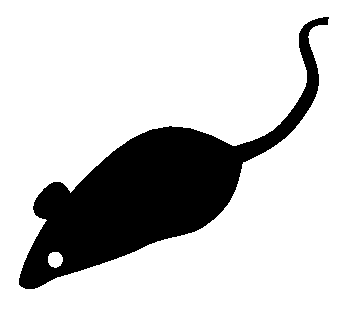
\includegraphics{mouse}
  \caption{Code before preprocessing.}
  \label{fig:one}
\end{figure}

\subsection{Problem Formulation}

The objective of variable coalescence-based offset assignment is to find
both the coalescence scheme and the MWPC on the coalesced graph. We start
with a few definitions and lemmas for variable coalescence.

% Enunciations
\begin{definition}[Coalesced Node (C-Node)]A C-node is a set of
live ranges (webs) in the AG or IG that are coalesced. Nodes within the same
C-node cannot interfere with each other on the IG. Before any coalescing is
done, each live range is a C-node by itself.
\end{definition}

\begin{definition}[C-AG (Coalesced Access Graph)]The C-AG is the access
graph after node coalescence, which is composed of all C-nodes and C-edges.
\end{definition}

\begin{lemma}
The C-MWPC problem is NP-complete.
\end{lemma}
\begin{proof} C-MWPC can be easily reduced to the MWPC problem assuming a
coalescence graph without any edge or a fully connected interference graph.
Therefore, each C-node is an uncoalesced live range after value separation
and C-PC is equivalent to PC. A fully connected interference graph is made
possible when all live ranges interfere with each other. Thus, the C-MWPC
problem is NP-complete.
\end{proof}

\begin{lemma}[Lemma Subhead]The solution to the C-MWPC problem is no
worse than the solution to the MWPC.
\end{lemma}
\begin{proof}
Simply, any solution to the MWPC is also a solution to the
C-MWPC. But some solutions to C-MWPC may not apply to the MWPC (if any
coalescing were made).
\end{proof}

\section{Performance Evaluation}

During all the experiments, the Geographic Forwarding (GF) by Akyildiz
et al.~\shortcite{Akyildiz-01} routing protocol is used. GF exploits
geographic information of nodes and conducts local data-forwarding to
achieve end-to-end routing. Our simulation is configured according to
the settings in Table~\ref{tab:one}. Each run lasts for 2 minutes and
repeated 100 times. For each data value we present in the results, we
also give its 90\% confidence interval.

% Table
\begin{table}%
\caption{Simulation Configuration}
\label{tab:one}
\begin{minipage}{\columnwidth}
\begin{center}
\begin{tabular}{ll}
  \toprule
  TERRAIN\footnote{This is a table footnote. This is a
    table footnote. This is a table footnote.}   & (200m$\times$200m) Square\\
  Node Number     & 289\\
  Node Placement  & Uniform\\
  Application     & Many-to-Many/Gossip CBR Streams\\
  Payload Size    & 32 bytes\\
  Routing Layer   & GF\\
  MAC Layer       & CSMA/MMSN\\
  Radio Layer     & RADIO-ACCNOISE\\
  Radio Bandwidth & 250Kbps\\
  Radio Range     & 20m--45m\\
  \bottomrule
\end{tabular}
\end{center}
\bigskip\centering
\footnotesize\emph{Source:} This is a table
 sourcenote. This is a table sourcenote. This is a table
 sourcenote.

 \emph{Note:} This is a table footnote.
\end{minipage}
\end{table}%


\section{Conclusions}

In this article, we develop the first multifrequency MAC protocol for
WSN applications in which each device adopts a
single radio transceiver. The different MAC design requirements for
WSNs and general wireless ad-hoc networks are
compared, and a complete WSN multifrequency MAC design (MMSN) is
put forth. During the MMSN design, we analyze and evaluate different
choices for frequency assignments and also discuss the nonuniform
back-off algorithms for the slotted media access design.

% Start of "Sample References" section

\section{Typical References in New ACM Reference Format}
A paginated journal article \cite{Abril07}, an enumerated
journal article \cite{Cohen07}, a reference to an entire issue \cite{JCohen96},
a monograph (whole book) \cite{Kosiur01}, a monograph/whole book in a series (see 2a in spec. document)
\cite{Harel79}, a divisible-book such as an anthology or compilation \cite{Editor00}
followed by the same example, however we only output the series if the volume number is given
\cite{Editor00a} (so Editor00a's series should NOT be present since it has no vol. no.),
a chapter in a divisible book \cite{Spector90}, a chapter in a divisible book
in a series \cite{Douglass98}, a multi-volume work as book \cite{Knuth97},
an article in a proceedings (of a conference, symposium, workshop for example)
(paginated proceedings article) \cite{Andler79}, a proceedings article
with all possible elements \cite{Smith10}, an example of an enumerated
proceedings article \cite{VanGundy07},
an informally published work \cite{Harel78}, a doctoral dissertation \cite{Clarkson85},
a master's thesis: \cite{anisi03}, an online document / world wide web
resource \cite{Thornburg01, Ablamowicz07, Poker06}, a video game (Case 1) \cite{Obama08} and (Case 2) \cite{Novak03}
and \cite{Lee05} and (Case 3) a patent \cite{JoeScientist001},
work accepted for publication \cite{rous08}, 'YYYYb'-test for prolific author
\cite{SaeediMEJ10} and \cite{SaeediJETC10}. Other cites might contain
'duplicate' DOI and URLs (some SIAM articles) \cite{Kirschmer:2010:AEI:1958016.1958018}.
Boris / Barbara Beeton: multi-volume works as books
\cite{MR781536} and \cite{MR781537}.

A couple of citations with DOIs: \cite{2004:ITE:1009386.1010128,
  Kirschmer:2010:AEI:1958016.1958018}.

Online citations: \cite{TUGInstmem, Thornburg01, CTANacmart}.

% Appendix
\appendix
\section{Switching Times}

In this appendix, we measure the channel switching time of Micaz
\cite{CROSSBOW} sensor devices.  In our experiments, one mote
alternatingly switches between Channels~11 and~12. Every time after
the node switches to a channel, it sends out a packet immediately and
then changes to a new channel as soon as the transmission is finished.
We measure the number of packets the test mote can send in 10 seconds,
denoted as $N_{1}$. In contrast, we also measure the same value of the
test mote without switching channels, denoted as $N_{2}$. We calculate
the channel-switching time $s$ as
\begin{displaymath}%
s=\frac{10}{N_{1}}-\frac{10}{N_{2}}.
\end{displaymath}%
By repeating the experiments 100 times, we get the average
channel-switching time of Micaz motes: 24.3\,$\mu$s.

\section{Supplementary Materials}


\begin{printonly}
  See the supplementary materials in the online version
\end{printonly}

\begin{screenonly}
\subsection{This is an Example of Appendix Subsection Head}

Channel-switching time is measured as the time length it takes for
motes to successfully switch from one channel to another. This
parameter impacts the maximum network throughput, because motes
cannot receive or send any packet during this period of time, and it
also affects the efficiency of toggle snooping in MMSN, where motes
need to sense through channels rapidly.

By repeating experiments 100 times, we get the average
channel-switching time of Micaz motes: 24.3 $\mu$s. We then conduct
the same experiments with different Micaz motes, as well as
experiments with the transmitter switching from Channel 11 to other
channels. In both scenarios, the channel-switching time does not have
obvious changes. (In our experiments, all values are in the range of
23.6 $\mu$s to 24.9 $\mu$s.)

\subsection{Appendix Subsection Head}

The primary consumer of energy in WSNs is idle listening. The key to
reduce idle listening is executing low duty-cycle on nodes. Two
primary approaches are considered in controlling duty-cycles in the
MAC layer.

\end{screenonly}

\begin{acks}

The authors would like to thank Dr. Maura Turolla of Telecom
Italia for providing specifications about the application scenario.

The work is supported by the \grantsponsor{GS501100001809}{National
  Natural Science Foundation of
  China}{http://dx.doi.org/10.13039/501100001809} under Grant
No.:~\grantnum{GS501100001809}{61273304\_a}
and~\grantnum[http://www.nnsf.cn/youngscientists]{GS501100001809}{Young
  Scientists' Support Program}.


\end{acks}

% Bibliography
\bibliographystyle{ACM-Reference-Format}
\bibliography{sample-bibliography}


%%%%%%%%%%%%%%%%%%%%%%%%%%%%%%%%%%%%%%%%%%%%%%%%%%%%%%%%%%%%%%%%%%%%%%%%%%%%%%%%%%%%%%%%%%%%%%%%%%%%%%%%%%%%%%%%%%%%
\section{Introduction}

	Fast development of Non-Volatile Memories(NVMs) bring exciting growth point to both of academic research and industrial production in the storage area. The representative NVMs are phase change memory\cite{Wong2010Phase}, STT-RAM\cite{Wang2013Low}, memristor\cite{Zangeneh2014Design} and Intel's 3D XPoint\cite{3dxpoint}. These NVM mediums provide byte-addressability, persistence, high-density and DRAM-like read and write performance. In order to utilizing the unique features of NVM, many recent researches have been proposed from different levels, such as persistent memory file system\cite{dulloor2014system,Zheng2017HMVFS,Volos2013Storage,condit2009better,wu2011scmfs,Ou2016A}, persistent memory key-value store system\cite{203265} and the novel programming models\cite{Hwang2015HEAPO,volos2011mnemosyne,zhang2015mojim} on persistent memory. These researches supply different management methods and various user interfaces for utilizing NVM. Besides the NVM-aware file systems, the NVM-aware NoSQL database systems have also attracting much research attention recently. As a main kind of NoSQL database system, several NVM-based key-value store systems and closely-related data structures\cite{echo,203265,Wu2016NVMcached,Oukid2016FPTree,nv-tree} are proposed for exploring persistent and consistent key-value store service on NVM. These systems mainly focus on the design method on the single-node architecture and solve the problem of persistent and consistent storage of key-value pairs on NVM, but can not well-adopt for the distributed environment applications in modern data centers. At the time, another technology called RDMA brings new opportunity to construct a high-throughput and low-latency distributed key-value store system by combing both NVM and RDMA.
	\par Remote Direct Memory Access(RDMA) is a mature direct memory access technology that enables directly accessing memory on a remote machine through specialized network without involving the remote CPU. RDMA can provide low latency, high bandwidth, low CPU utilization and has been widely adopted in high performance computing environments for decades. Although RDMA is not a novel technology, the recently emerging NVM technology makes it popular again, because the combination of RDMA and NVM will introduce attractive features for fast and low-latency memory storage. These features will supply great benefit for date-intensive applications in the modern data centers. For key-value store system, it offers an special opportunity to construct a distributed, RDMA-enabled, completely in-memory key-value storage system with both data persistence and consistence. State-of-the-art in-memory key-value stores often backup their in-memory data to disk to provide durability. However,the latency and bandwidth gap between disk and DRAM makes it impossible to backup data synchronously. For example, Redis\cite{redis} and RAMCloud\cite{rumble2014log} periodically flush data to disks or SSDs in a user specified time interval, which means the data will be lost if a power failure occurred during this period. The emerging byte-addressable NVM technologies have a comparable read/write latency to DRAM, which makes it an attractive replacement for DRAM and Disk/SSD solution. However, the consistency and fault-tolerance problem for distributed key-value store system still needed to be optimized further. For instance, in a distributed key-value store system, a key-value pair often has several replications, when a server crashed or became inaccessible because of network disconnection, backup servers could still serve requests. PBR with N replications can tolerate N - 1 server failure. Suppose the average crash probability of a server is P(P << 1), then the unavailability of a N replicated storage system equals to PN. In traditional DRAM + Disk/SSD key-value stores with primary backup, the replication procedure is as follows. The primary server first writes to local storage, and then sends request to N - 1 backup servers, it sends response to the client after having received all responses from N - 1 backup servers. By this approach, a request needs to be  executed at	N independent servers, which results in great CPU resource waste and several times of higher latency. When replacing DRAM and Disk/SSD with NVM, the persistency time is	decreased, but the time cost and CPU usage of re-executing the request at backup servers remain if we follow the same replication procedure. In order to reduce the average latency of key-value pair persistent process, we leverage the RDMA technology to realize a distributed low-latency key-value store on NVM named DoubleM-KV. 
	\par In DoubleM-KV, we propose a byte-to-byte replication scheme utilizing one-sided RDMA write of infiniband fabric. For a PUT	request, we first execute the request in primary server, which introduces several data and metadata writes to local NVM. These NVM modifications are then collected and replicated to the same address of backup servers' NVM storage by one-sided RDMA write. In our approach, the re-execution of requests are eliminated, which significantly decreases the replication latency and backup server's CPU usage, because one-sided RDMA write does not invoke the backup servers' CPU. 
		
	\noindent The technical contribution of this paper can be illustrated as follows:

	\begin{itemize}
		\item We design a fast replication mechanism which is optimized for NVM over RDMA fabric.
		\item We implemented a distributed key-value store prototype called DoubleM-KV. We conducted experiments on Mellanox ConnectX-3 NIC to evaluate the performance of our design. Experimental results show that a replication of 32 bytes PUT request to 2 backup servers completes in only around 2$\upmu$s.
		\item To overcome the limitation of traditional key-value stores, we first explores the design of a distributed low-latency key-value store on non-volatile main memory by leveraging RDMA. 
	\end{itemize}

	The remainder of this paper is structured as follows. The following section briefly introduces key/value stores, NVM and RDMA. Section III presents our design and describes the replication approach. Section IV shows several importantimplementation details of NVDS. In Section V, we evaluate our work on servers equipped with Mellaonx infiniband. Finally, we conclude our paper in Section VII.

	
	

	

	

	
	
	
	
\section{Motivation and Background}

\subsection{Non-Volatile Memory}	
	
	

\subsection{Remote Direct Memory Access}
	

\subsection{Distributed Key-Value Store}
	
	
	
\section{DoubleM-KV Design}



\section{Implementation}

	

\section{Evaluation}


\section{Related Work}
	

\section{Conclusion}
	
	
	
	
	
%%%%%%%%%%%%%%%%%%%%%%%%%%%%%%%%%%%%%%%%%%%%%%%%%%%%%%%%%%%%%%%%%%%%%%%%%%%%%
\section*{Acknowledgement}


%%%%%%%%%%%%%%%%%%%%%%%%%%%%%%%%%%%%%%%%%%%%%%%%%%%%%%%%%%%%%%%%%%%%%%%%%%%%%
% Bibliography
\bibliographystyle{ACM-Reference-Format}
\bibliography{thesis}


\end{document}
